\section{Hierarchia nierozstrzygalności}

\subsection{Maszyna z wyrocznią}
Dla języka \(A\) maszyna \(T^A\) oznacza maszynę z wyrocznią dla języka \(A\). Wyrocznia ma własność STOP a zapytania są wykonywane w czasie \(\bigO(1)\).

Język \(L\) jest w klasie \(\re \ (\rec)\) z wyrocznią dla \(A\), gdy \(L = L(T^A)\) dla maszyny \(T^A\) \\ (z własnością STOP).

Dla języków \(L_1, L_2 \subseteq \Sigma^*\) definiujemy relację równoważności:
\[ L_1 \approx L_2 \text{ wtw } L_1 \text{ jest rekurencyjny z wyrocznią } L_2 \text{ i vice versa} \]

\subsection{Hierarchia}
Coraz głębsze warstwy nierozstrzygalności:
\begin{align*}
    S_1 & = \set{\langle M \rangle : L(M) = \emptyset} \approx L_e \\
    S_2 & = \set{\langle M^{S_1} \rangle : L(M^{S_1}) = \emptyset} \\
    & \approx \set{\langle M \rangle : L(M) = \Sigma^*} \\
    & \dots
\end{align*}
Kolejne warstwy korzystają z wyroczni dla poprzednich.

Dla każdego \(i \geq 1\), \(S_{i+1}\) nie jest \(\re\) ze względu na \(S_i\).

\newpage
\begin{theorem}
    \(L_u \approx L_e\)
\end{theorem}
\begin{proof}
    \textit{Algorytm dla \(L_U\) przy wyroczni \(L_e\)} \\
    Konstruujemy maszynę \(M'\), która akceptuje \(\Sigma^*\), jeśli \(w \in L(M)\) i nic, wpp. Testujemy \(M'\), zapytując wyrocznię dla \(L_e\). W ten sposób rekurencyjnie rozpoznajemy \(L_U\).

    \textit{Algorytm dla \(L_e\) przy wyroczni \(L_U\)} \\
    Konstruujemy maszynę \(M'\) taką, że albo \(L(M) = L(M') = \emptyset\), albo \(L(M) \neq \emptyset\) i \(L(M') = \Sigma^*\). \\
    Iterując po parach \((i,j)\), symulujemy \(j\) kroków \(M\) na \(i\)-tym słowie. Jeśli \(M\) zaakceptuje jakieś słowo, \(M'\) akceptuje słowo \(w'\) na wejściu, wpp \(M'\) się pętli.

    Maszyna \(M_U\) rozpozna \((\langle M' \rangle, w')\) wtw, gdy \(L(M) \neq \emptyset\).
\end{proof}

\begin{theorem}
    \( S_2 = \set{\langle M^{S_1} \rangle : L(M^{S_1}) = \emptyset} \approx \set{\langle M \rangle : L(M) = \Sigma^*} \)
\end{theorem}
\begin{proof}[Dowód rekurencyjności \(\geq\)]\textcolor{white}{\\}
    Konstruujemy pisarza \(C\), który zwraca kod maszyny \(M^{L_u}\), korzystającej z wyroczni \(L_u\).
    \begin{figure}[H]
        \centering
        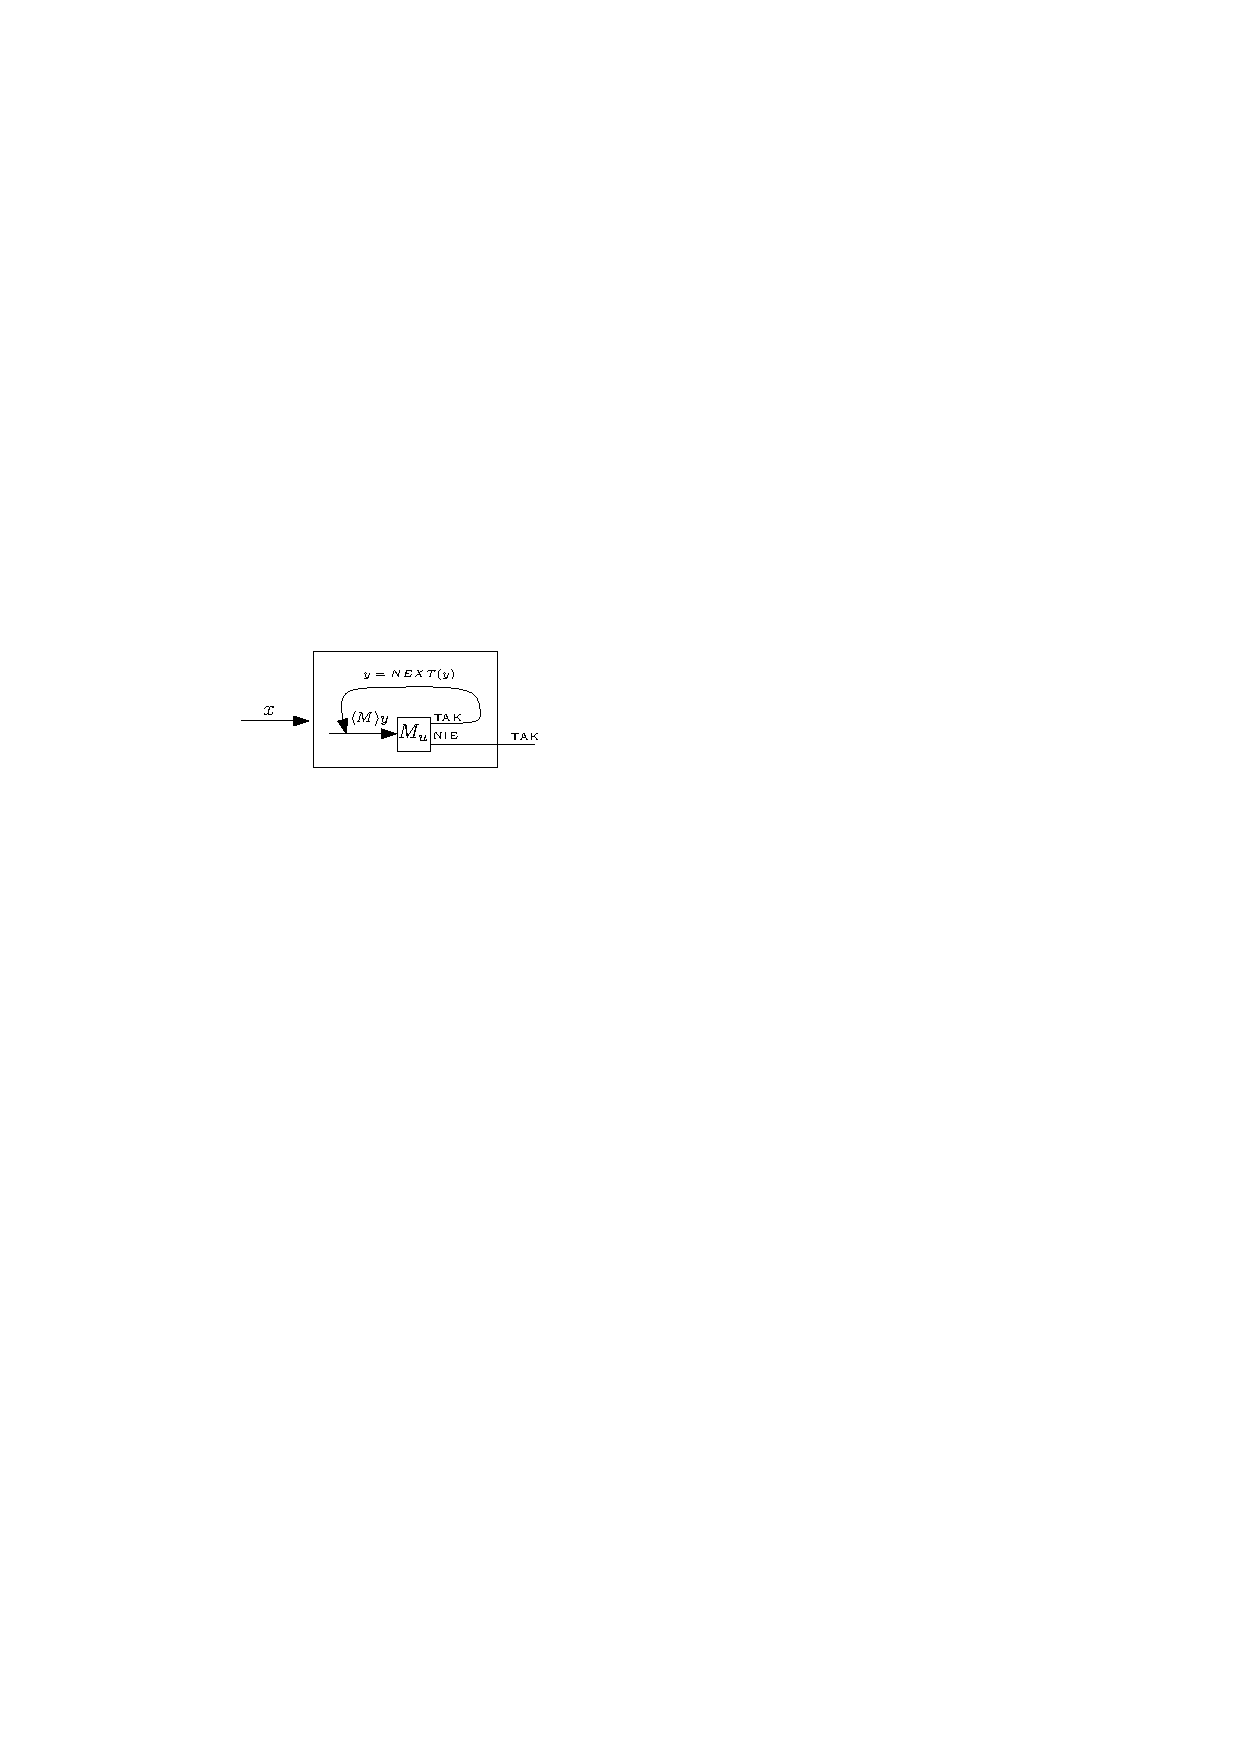
\includegraphics[width=0.4\linewidth]{img/Mlu.pdf}
    \end{figure}
    Następnie konstruujemy maszynę z wyrocznią dla \(S_1\), która sprawdza, czy język maszyny jest pełny.
    Korzystamy z tego, że \(L_u \approx S_1\), więc możemy podmienić wyrocznie \(L_u\) na wyrocznię \(S_1\). 
    \begin{figure}[H]
        \centering
        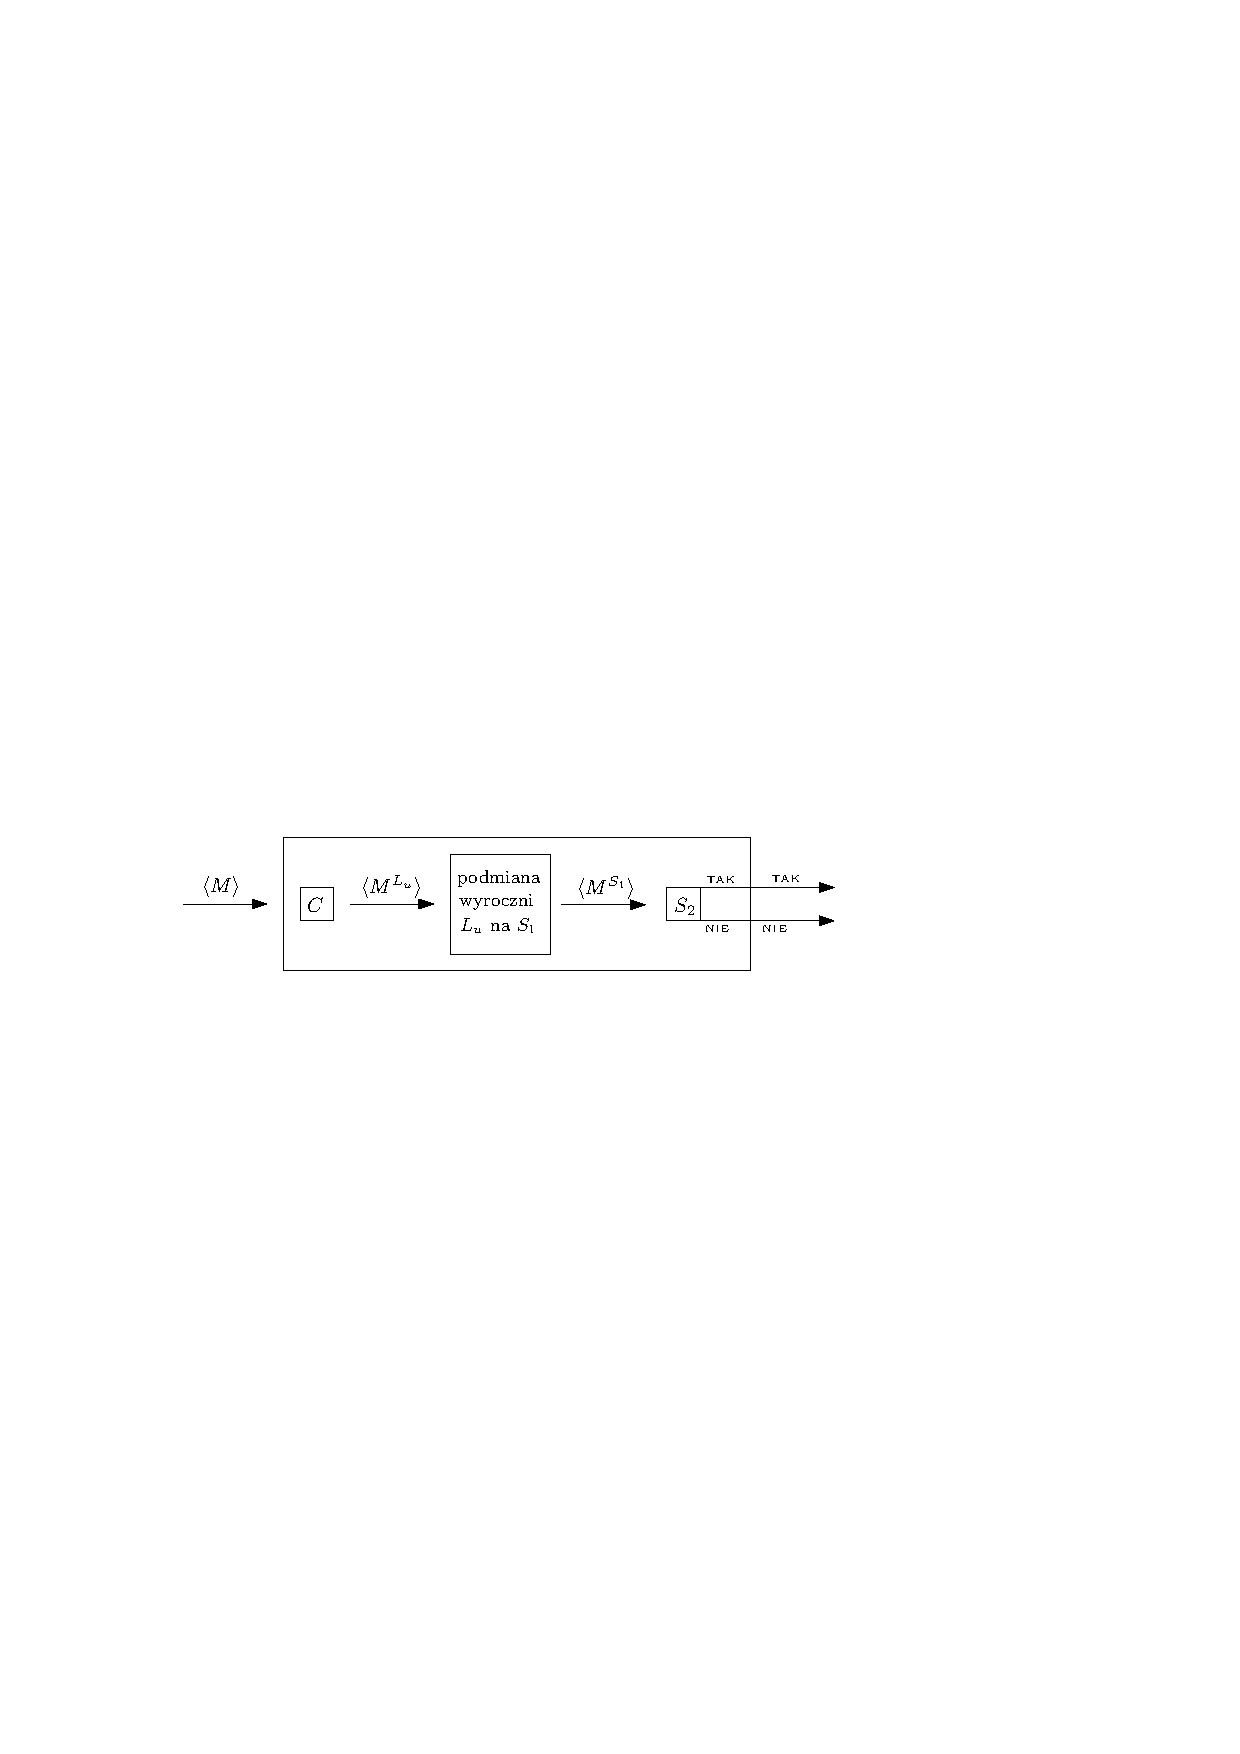
\includegraphics[width=0.7\linewidth]{img/wyrocznia2.pdf}
    \end{figure}
    \begin{itemize}
        \item[I] Jeśli \(L(M)=\Sigma^*\), to \(L(M^{S_1})=\emptyset\), więc maszyna akceptuje.
        \item[II] Jeśli \(L(M)\neq\Sigma^*\), to \(L(M^{S_1})=\Sigma^*\), więc maszyna nie akceptuje.
    \end{itemize}
\end{proof}
